\documentclass[11pt]{iopart}

\usepackage{graphicx}
\usepackage{epsf}
\usepackage{longtable}
\usepackage{hyperref}
\usepackage{graphics,epsfig,placeins,subfigure,wrapfig}
\expandafter\let\csname equation*\endcsname\relax

\expandafter\let\csname endequation*\endcsname\relax
\usepackage{amsmath,amssymb,calc,amsfonts}
\usepackage[usenames]{color}
\usepackage{soul}
\usepackage{amsfonts}
\usepackage[mathscr]{euscript}

\DeclareMathAlphabet\mathbfcal{OMS}{cmsy}{b}{n}

\def\eadnew#1#2{\address{#2 E-mail: \mailto{#1}}} 

\begin{document}

\title{Modelado matemático I}

\author{Jesús Andrés Arrieta Villamizar $-$ 2208058}
\address{$^1$  Escuela de F\'isica, Universidad Industrial de Santander.}

\section*{El juego de la vida}

En el presente documento se explicará de manera breve la forma en que se llevó a cabo la programación del juego de la vida. En primera instancia, es necesario mencionar las reglas bajo las cuales se rige:
%
\begin{enumerate}
\item Una célula muerta con exactamente 3 células vecinas vivas “nace” (es decir, al turno siguiente estará viva).
\item Una célula viva con 2 o 3 células vecinas vivas sigue viva, en otro caso muere (por “soledad” o “superpoblación”).
\end{enumerate}

En primera instancia, se creó el lienzo sobre el cual se desarrolla el juego, es decir, una matriz aleatoria llena de unos y ceros, donde $0 = $ persona muerta, mientras que $ 1 = $ persona viva. Para definir la forma de evolución de la población inicial, se realizó una traslación de las diferentes casillas del tablero y así poder contar cuántos vecinos vivos y muertos tiene cada casilla. En la figura \eqref{fg:rb}(imagen izquierda)  se muestra el algoritmo implementado para realizar el análisis de cada vecino mendiante la traslación de las casillas; dichos desplazamientos contemplan los vecinos: superior $(roll_{u})$, inferior $(roll_{d})$, a izquierda $(roll_{l})$, a derecha $(roll_{lr})$, diagonales superiores a izquierda y derecha $(roll_{lu}, \, roll_{ru})$ y diagonales inferiores a izquierda y derecha $(roll_{ld}, \, roll_{rd})$. 
%
\\
\begin{figure}[h!]
\centering
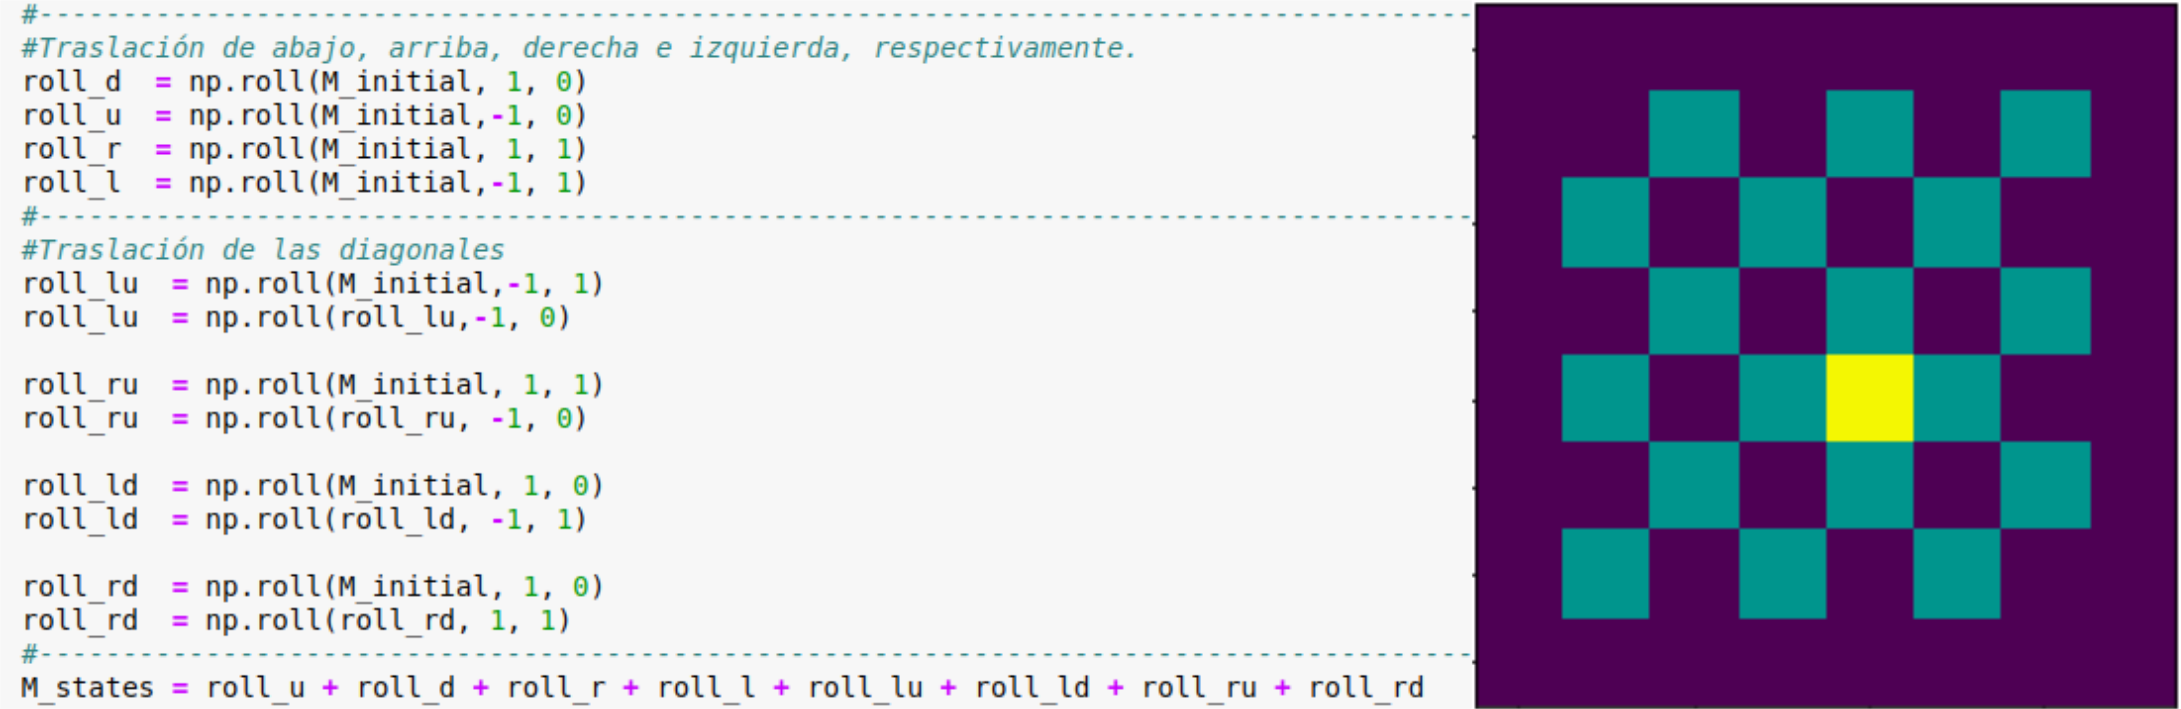
\includegraphics[width = 0.75\textwidth]{Figs/roll_board}
\caption{Algoritmo y representación gráfica del desplazamiento de las casillas de la matriz inicial. En la figura de la izquierda se muestra el algoritmo con el que se realizaron los diferentes desplazamientos para una celda genérica. A la derecha, en la población inicial, la celda en amarillo permite visuaizar cómo se desplaza una celda desde una posición inicial $[i_{0}, j_{0}]$, a una posición final $[i_{f}, j_{f}]$, donde $i , j$ representan las filas y columnas, respectivamente\label{fg:rb}}
\end{figure}
\\
%
Adicionalmente, se muestra una representación gráfica (imagen derecha) de una población inicial. Esta última, para efectos ilustrativos, se escogió de manera simétrica, como un tablero de ajedrez, y se seleccionó una casilla en color amarillo para mostrar la forma en que podía realizarse una traslación de una casilla de su posición inicial a otra casilla en una posición deseada. Puede verse que los bordes solo tienen personas muertas; esto se hizo con la intención de evitar problemas de frontera durante la evolución de la población a medida que transcurre el juego. 
\\ \\
Por otra parte, para seleccionar el estado de cada celda en la matriz de población, se creo una matriz $M_{states}$ como la suma de todas las traslaciones. El resultado de esta, es que en  alguna posición que se desee conocer, la matriz $M_{states}$ provee el número de vecinos que tiene cada celda de la matriz original, con esto es posible aplicar las reglas establecidas por el juego y así se define si alguna célula en cuestión vive, muere o se mantiene en un estado constante. Una vez establecido el lienzo sobre el cual interactúa la población, se procede a evolucionarla para un instante inicial $t_{0}$. En la figura \eqref{fg:evolution}, se muestra el algoritmo con el cual se evolucionó la población inicial, y como resultado, se obtiene una nueva generación de personas. Cada generación al salir de un ciclo evolutivo se denominó $\Gamma$.
%
\begin{figure}[h!]
\centering
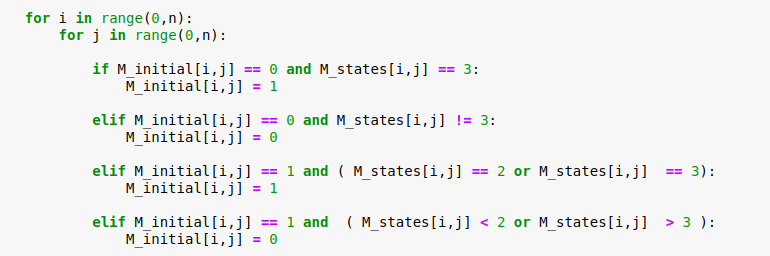
\includegraphics[width = 0.9\textwidth]{Figs/evolution}
\caption{Algoritmo para la evolución de la población inicial. Se observa cómo mediante un ciclo $for$ anidado, se recorre la posición de cada celda y se compara con la matriz de estados con cuatro condiciones distintas, que son las reglas previamente establecidas para el juego. Como retorno de este bucle iterativo, se obtiene una nueva matriz cuyos elementos representan las nuevas personas vivas y muertas. \label{fg:evolution}}
\end{figure}
\\ 
%
Una vez definida la evolución de la población inicial $\Gamma = 0$, se creó uno nuevo ciclo iterativo que permitiera visualizar la distribución de personas vivas y muertas de una generación a otra. En la figura \eqref{fg:final} se  presenta el algoritmo que realiza lo anteriormente mencionado, que en términos de imágenes, representará el número de figuras que conforman el video del juego (archivo adjunto en esta carpeta). Adicionalmente, se muestra un ejemplo con $\Gamma = 20$, en el cual puede apreciarse cómo de una población inicial $\Gamma = 0$, con gran cantidad de personas vivas, el resultado final muestra un decaimiento de dicha distribución de personas.
%
\begin{figure}[h!]
\centering
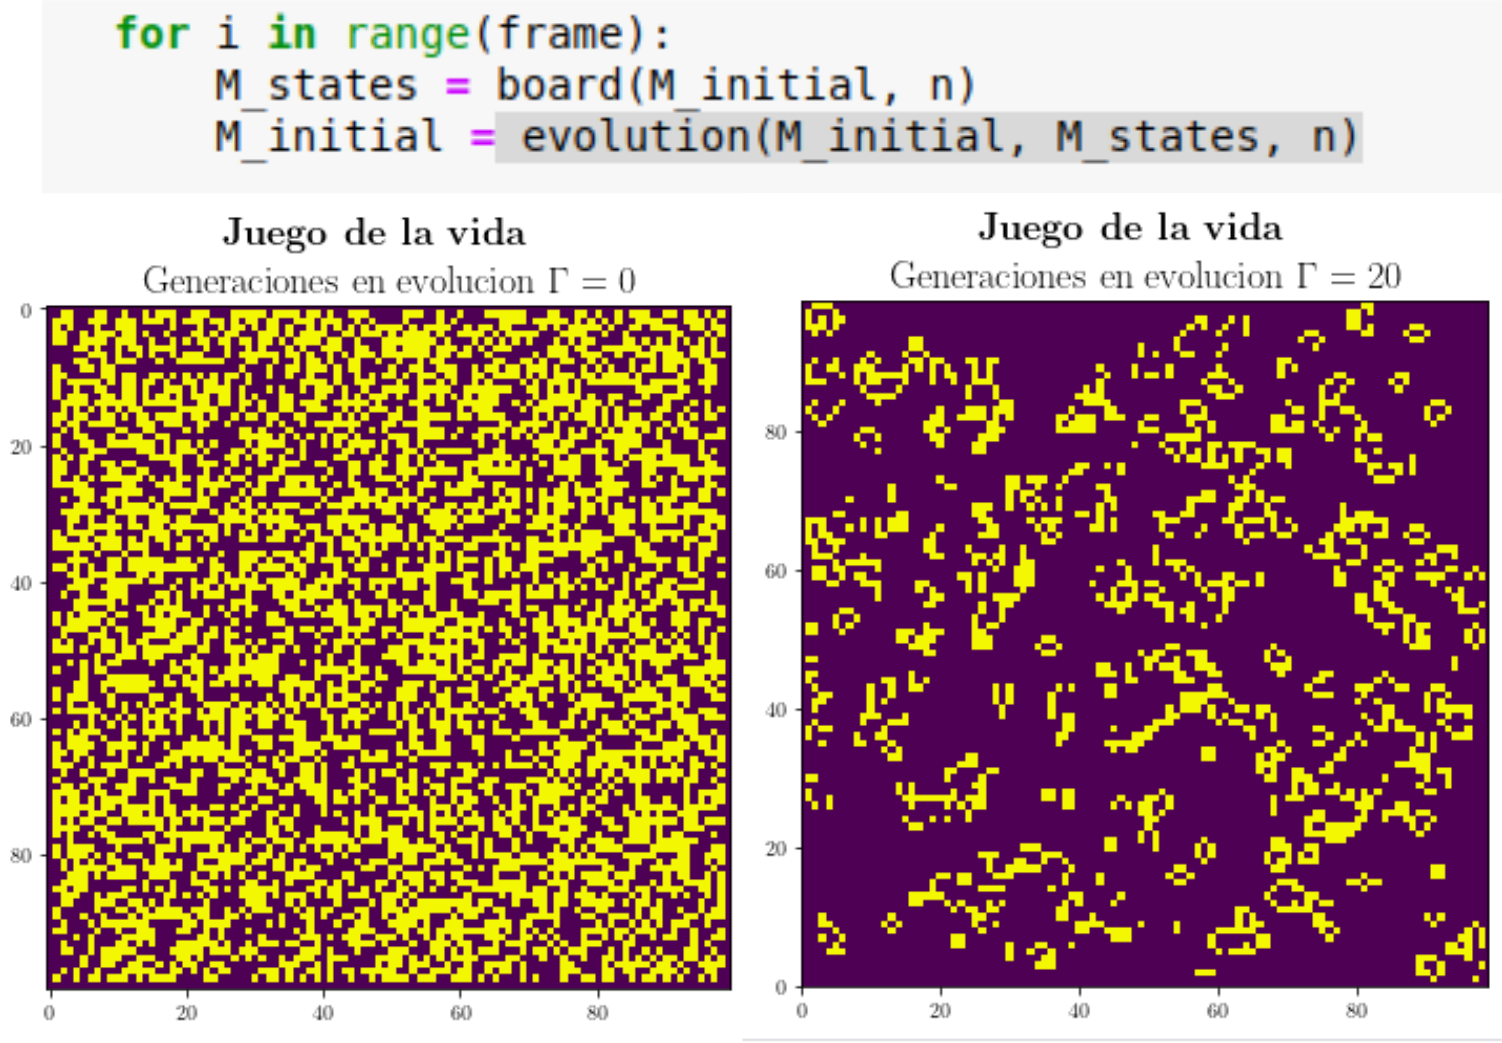
\includegraphics[width = 0.9\textwidth]{Figs/final}
\caption{Algoritmo para la evolución entre generaciones. En la figura izquierda, se observa la población inicial (creada mediante una matriz aleatoria), correspondiente con $\Gamma = 0$. Los puntos amarillos y morados resprentan las personas vivas y muertas de dicha distribución. En la imagen derecha, se puede apreciar el resultado final luego de evoluciar 20 generaciones, cuyo resultado es una clara disminución de las personas vivas.  \label{fg:final}}
\end{figure}
%
\end{document}